\documentclass{beamer}

\mode<presentation>
{
\usetheme{Dresden} 
%\usecolortheme{spruce}
\usefonttheme{professionalfonts}
%\setbeamercovered{invisible}
%\setbeamertemplate{itemize subitem}[triangle]
\setbeamertemplate{blocks}[rounded]
\setbeamertemplate{footline}
{
  \leavevmode%
  \hbox{%
  \begin{beamercolorbox}[wd=.25\paperwidth,ht=2.25ex,dp=1ex,left]{title in head/foot}%
    \usebeamerfont{author in head/foot}\hspace*{2ex}\insertauthor
  \end{beamercolorbox}%
  \begin{beamercolorbox}[wd=.5\paperwidth,ht=2.25ex,dp=1ex,center]{date in head/foot}%
    \usebeamerfont{title in head/foot}\inserttitle
  \end{beamercolorbox}%
  \begin{beamercolorbox}[wd=.175\paperwidth,ht=2.25ex,dp=1ex,right]{title in head/foot}%
    \usebeamerfont{date in head/foot}\insertshortdate{} \hspace*{2ex}
  \end{beamercolorbox}}%
  \begin{beamercolorbox}[wd=.075\paperwidth,ht=2.25ex,dp=1ex,center]{date in head/foot}%
    \insertframenumber{} / \inserttotalframenumber
  \end{beamercolorbox}%
  \vskip0pt%
}
}

\usepackage{amsmath}
\usepackage{amsfonts}
\usepackage{graphicx}
\usepackage[english]{babel}
\usepackage[utf8]{inputenc}
\usepackage[T1]{fontenc}
\usepackage{multirow}
\usepackage{rotating}
\usepackage[scaled=.90]{helvet}
\usepackage{xcolor}
\usepackage[T1]{fontenc}
\usepackage{abbrevs}


\beamertemplatenavigationsymbolsempty
\setbeamerfont{footnote}{size=\tiny}
\setbeamertemplate{itemize subitem}[triangle]


\title{A critical review of age-related research on L2 ultimate attainment}
\author{A. Wachtler and C. Jenkins}
\institute{Institut f\"ur Maschinelle Sprachverarbeitung, Universit\"at Stuttgart\\Probabilistic Graphical Models for Natural Language Processing}
\date{6 July 2016}

\begin{document}

\AtBeginSection[]{
  \begin{frame}
  \vfill
  \centering
  \begin{beamercolorbox}[sep=8pt,center,shadow=true,rounded=true]{title}
    \usebeamerfont{title}\insertsectionhead\par%
  \end{beamercolorbox}
  \vfill
  \end{frame}
}


% Cover Page
\begin{frame}
  \titlepage
\end{frame}

% Outline
 \begin{frame}{Outline}
   \tableofcontents
 \end{frame}

\begin{frame}{Recap - last week}
    % dealing with difficulties in studying SLA
    % use of a computational model to create a well-defined, controlled situation
    The Bilingual Language Interaction Network for Comprehension of Speech.
    \begin{itemize}
      \item Problem: 2nd Language acquisition has many factors
      \item These are difficult to control for in experimental groups 
      \\
      \item Approach: computational model of bilingualism
      \begin{itemize}
        \item BLINCS model
        \item Operates at semantic, phonological, lexical, orthographic levels
        \item Incorporates L1 knowledge
      \end{itemize}
    \end{itemize}
\end{frame}

\begin{frame}{This week's paper}
    \begin{center}
        A critical review of age-related research on L2 ultimate attainment \\
        By Carmen Muñoz and David Singleton \\
        Appeared in Language Teaching vol. 44
    \end{center}
\end{frame}

\section{Overview}

\begin{frame}{Prelude to a Contentious Topic}
  \begin{itemize}
    \item The authors offer some good advice:
    \begin{itemize}
      \item Respect your colleagues
      \item Even if you diasgree with their approach
      \item Science is a laborious process
    \end{itemize}
  \end{itemize}
\end{frame}

\begin{frame}{Main Questions}
  \begin{itemize}
    \item Is there a window (around end of childhood) after which language acquisition is \emph{qualitatively} different?
    \begin{itemize}
      \item Clearly the case with acquiring L1
    \end{itemize}
    \item Are other factors more relevant to decline in language acquisition ability?
    \item Are changes in the brain overstated?
  \end{itemize}
\end{frame}

\section{L1-Speaker Benchmark}

\begin{frame}
	\centering
	\Huge{What \textcolor{blue}{\textit{is}} a native speaker?}
\end{frame}

\begin{frame}
	\begin{itemize}
		\item Place of birth?
		\pause
		\item Time spent in country of L1?
		\pause
		\item What you identify yourself as?
		\pause
		\item The language you feel most comfortable with?
		\pause
		\item Current citizenship?
		\pause
		\item Cultural background?
		\pause
		\item L1 obtained during critical period?
	\end{itemize}
\end{frame}

\begin{frame}{Functional L1 switch}
	Success in L2 environment depends on age and involvement:
	\begin{itemize}
		\item Younger than 10 years of age
		\pause
		\begin{itemize}
			\item L1 accent modified by L2
			\item L2 becomes functional L1
		\end{itemize}
		\pause
		\item Older than 10 years of age
		\pause
		\begin{itemize}
			\item L1 strongly influences L2
			\item L1 further developes
			\item No functional switch
		\end{itemize}
	\end{itemize}
	\pause
	\vspace{0.25cm}
	Peer group important in L2 learning
\end{frame}

\begin{frame}{Late L1 learners}
	\begin{columns}
		\begin{column}{4cm}
			\includegraphics[scale=0.5]{tarzan}
		\end{column}
		\begin{column}{4cm}
			\includegraphics[scale=0.3]{deaf}
		\end{column}
	\end{columns}
\end{frame}

\begin{frame}{Limitations of post-pubertal L2 learning}
	Critical-period research argues that no late-L2-learner can achieve native-like proficiency:
	\pause
	\begin{itemize}
		\item Differences in accent
		\pause
		\item Lexicon
		\pause
		\item Grammar
		\pause
		\item Vowel \& consonant perception
	\end{itemize}
	\pause
	\vspace{0.25cm}
	$\rightarrow$ Knowledge of L1 \& distance to L2?
\end{frame}

\begin{frame}{Native speakers - unrealistic benchmark}
	For comparison, stay in one learning domain
	\pause
	\begin{itemize}
		\item Compare late to early L2 learners
		\pause
		\item Identify similar backgrounds
		\pause
		\item Age is important, critical period probably not so much
		\pause
		\item Not everyone tries to achieve native-like levels
	\end{itemize}
\end{frame}

\section{Definition(s) of Crit. Period}

\begin{frame}{Classic Definition}
  \begin{itemize}
    \item After age 9
    \begin{itemize}
      \item Penfield \& Roberts (1959)
    \end{itemize}
    \item After puberty
    \begin{itemize}
      \item Lenneberg (1967)
    \end{itemize}
    \item Already some disagreement
  \end{itemize}
\end{frame}

\begin{frame}{Additional Definitions}
  Different critical points for various components of language \\
  Ruben (1997)
  \begin{itemize}
    \item Phonetics / Phonology
    \begin{itemize}
      \item $\approx$ 12 months
      \item From studies of children with temporary hearing problems during 1st year
    \end{itemize}
    \item Syntax
    \begin{itemize}
      \item $\approx$ 4 years
    \end{itemize}
    \item Semantics
    \begin{itemize}
      \item $\approx$ 15-16 years
    \end{itemize}
  \end{itemize}
\end{frame}

\begin{frame}{Other Critical Periods}
  \begin{itemize}
    \item Bionocular vision
    \begin{itemize}
      \item Input from both eyes needed at a young age
      \item Clearly defined point
    \end{itemize}
    \item Imprinting
    \begin{itemize}
      \item Some bird species quickly learn to follow someone
      \item Ideally this is their parent
    \end{itemize}
    \item Ethical concerns
  \end{itemize}
\end{frame}

\begin{frame}{Dramatic Dropoff}
  \begin{itemize}
    \item ``Elbow shape'' dropoff?
    \begin{itemize}
      \item Severe difference in language learning ability
      \item \emph{Qualitative} difference
      \item DeKeyser, Alfi-Shabaty \& Ravid (2010)
      \begin{itemize}
        \item Rapid drop-off after age 18
      \end{itemize}
    \end{itemize}
    \item Gradual decline
    \begin{itemize}
      \item Age-related cognitive deterioration
      \item \emph{Linear} decline throughout life
      \item Bialystok \& Hakuta 1999; Flege 1999; Birdsong 2004, 2006
    \end{itemize}
  \end{itemize}
\end{frame}


\section{Contextual Factors}

\begin{frame}{Classic Benchmarks} % discussing Age of Acquisition, Length of Residence, pros, cons
    \begin{itemize}
        \onslide<2->\item Age of Acquisition (AoA)
        \onslide<3->\item Length of Residence (LoR) \\
       \onslide<4->\item Positive:
        \begin{itemize}
          \onslide<5->\item Easy to obtain
        \end{itemize}
       \onslide<6->\item Negative:
        \begin{itemize}
         \onslide<7->\item Much variation not accounted for
        \end{itemize}
        % moving beyond these
    \end{itemize}
\end{frame}

\begin{frame}{Social Factors} % this could really be several slides
  \begin{itemize}
    \item Exposure to language input can be limited by circumstances
    \begin{itemize}
      \item Even in a country where that language is predominantly spoken
    \end{itemize}
  \end{itemize}
  \onslide<2->\begin{columns}
    \column{0.5\textwidth}
      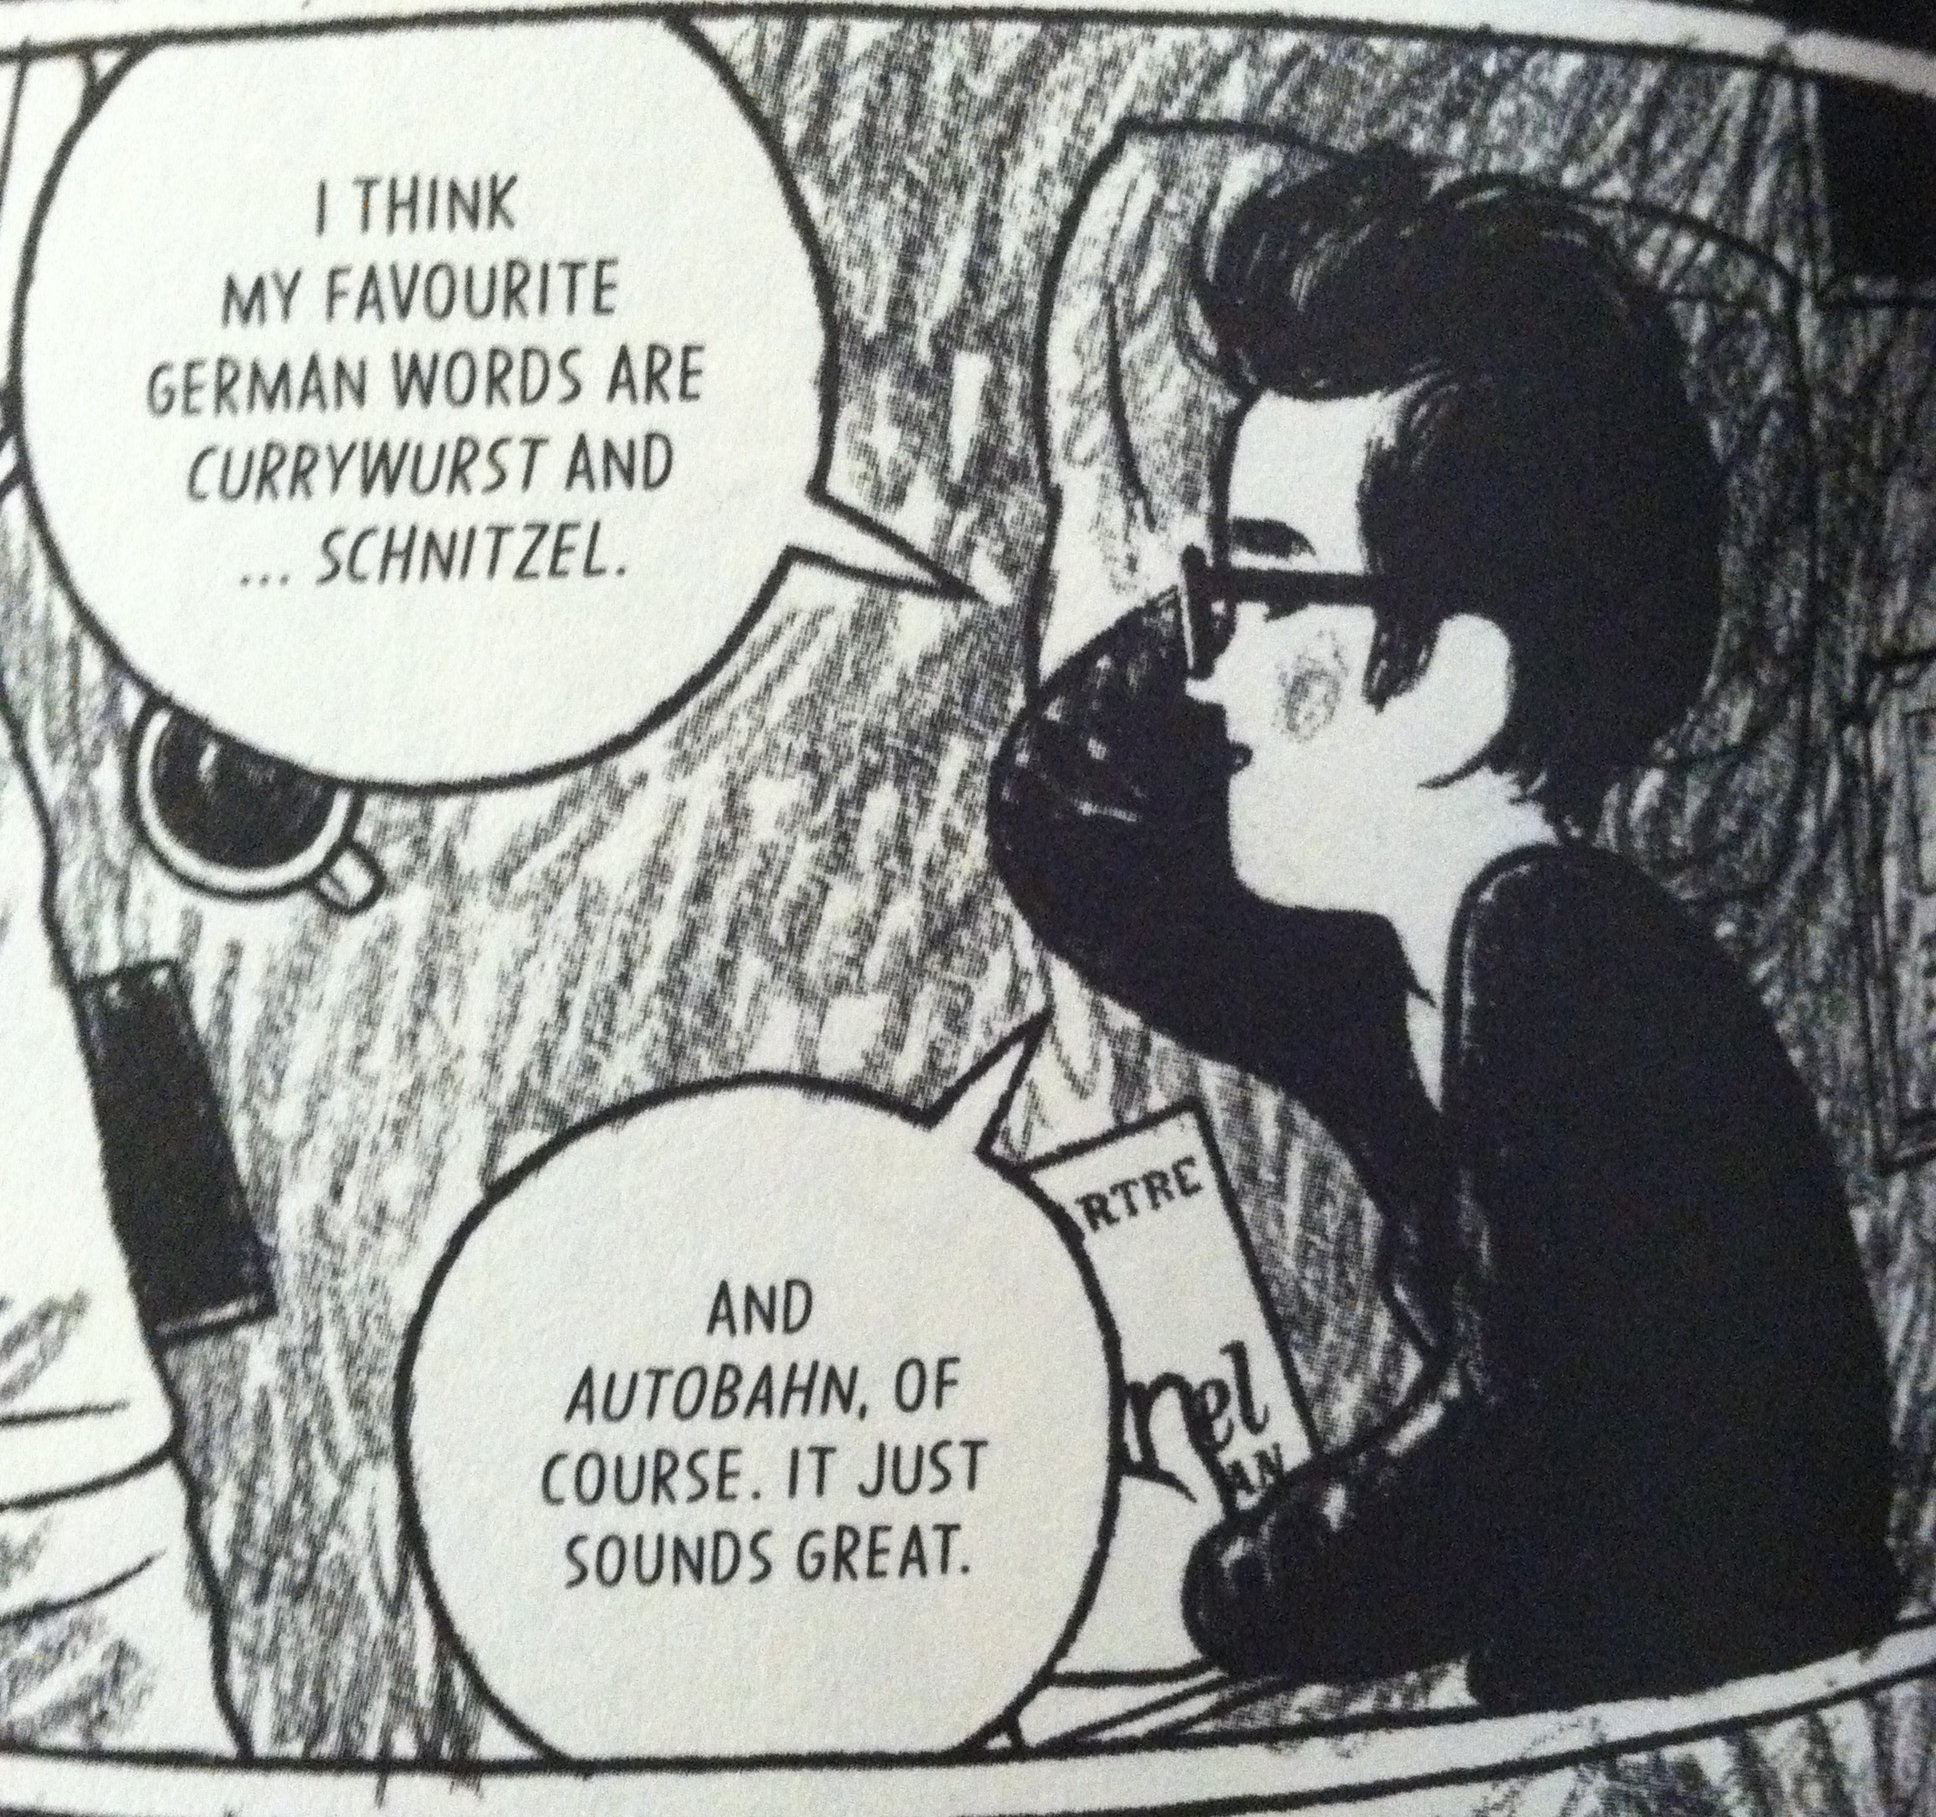
\includegraphics[scale=0.07]{currywurst_cropped.JPG} \\
      \tiny{\textit{Baby's in Black} by Arne Bellstorf}
    \column{0.5\textwidth}
      
\includegraphics[scale=0.05]{trash_detective.jpg}
  \end{columns}
\end{frame}

\begin{frame}{Social Factors}
  \begin{itemize}
    \item Social factors can affect \emph{exposure} to and \emph{use} of L2
    \begin{itemize}
      \item Often correlate with chronological age
    \end{itemize}
    \item Life as a student
    \item Language(s) spoken by colleagues, housemates, partners, etc
  \end{itemize}
\end{frame}


\begin{frame}{Feedback Loop}
  \begin{itemize}
    \item Language experience builds on experience
    \begin{itemize}
      \item More opportunities to have conversations
    \end{itemize}
    \item Earlier L2 learning could correspond to family, friend, community groups
    \item Confidence, sense of self
  \end{itemize}
\end{frame}

\begin{frame}{Identity}
  \begin{itemize}
    \item Tends to be more well-established with age
    \item Language can be a major factor of one's sense of self
  \end{itemize}
\end{frame}

\begin{frame}{Study Methodology}
    \begin{itemize}
        \item Interview Questions
        \begin{itemize}
          \item Self-reporting is \emph{difficult}
          \item Understanding subjects' day-to-day L2 contact
        \end{itemize}
        \item Longitudinal Studies
    \end{itemize}
\end{frame}

\begin{frame}{Section Summary}
  \begin{itemize}
    \item L2 learners who start earlier \emph{do} tend to have better outcomes
    \item Effect of age
    \begin{itemize}
      \item Neurological changes are perhaps overstated (Critical Period)
      \item Social changes understated
    \end{itemize}
  \end{itemize}
\end{frame}

\section{Neurolinguistic Considerations}

\begin{frame}{Differential Localization}
	\begin{itemize}
		\item Separation of L1 \& L2
		\pause
		\begin{itemize}
			\item L1 developes during critical period
			\item L2 uses brain areas not occupied with L1
			\item Effects of aphasia taken as proof
		\end{itemize}
		\pause
		\item Grammar acquistion/representation
			\begin{itemize}
				\item Implicit acquistion of L1 grammar during critical period
				\item L2 grammar declarative, but still unconscious
				\item L1 uses implicit processing, L2 memory-based
			\end{itemize}
	\end{itemize}
	\pause
	\vspace{0.25cm}
	$\rightarrow$ Possible brain changes after critical period
\end{frame}

\begin{frame}{Convergence Hypothesis}
	\begin{itemize}
		\item L1 defines cerebral structure
		\pause
		\item L2 aligns with neural language system of L1
		\pause
		\item System controlled by prefrontal cortex
		\pause
		\item Higher L2 proficiency $\rightarrow$ less prefrontal activity
	\end{itemize}
\end{frame}

\begin{frame}{Comments}
	\begin{itemize}
		\item Language proficiency relies on input (L1 \& L2 switch)
		\pause
		\item Influence of attrition \& relearning unclear
		\pause
		\item After critical period, sudden or gradual deterioration rate?
		\pause
		\item More longitudinal studies needed (avoid too much variability)
		\pause
		\item Lacking evidence of critical period
	\end{itemize}
\end{frame}

\section{Takeaway}

\end{document}
